\documentclass[12pt,a4paper]{article}
\usepackage[UTF8]{ctex}
\usepackage{geometry}
\usepackage{amsmath,amssymb,amsthm}
\usepackage{mathtools,bm}
\usepackage{empheq}
\usepackage{graphicx}
\usepackage{booktabs}
\usepackage[numbers,sort&compress]{natbib}
\usepackage{caption}
\usepackage{enumitem}
\usepackage{chngcntr}
\usepackage{tikz}

% ========== 页面布局 ==========
\geometry{left=2.5cm,right=2.5cm,top=2.5cm,bottom=2.5cm}
\setlength{\parskip}{0.5em}
\renewcommand{\baselinestretch}{1.2}

% ========== 数学命令 ==========
\newcommand{\diff}{\mathop{}\!\mathrm{d}}
\newcommand{\R}{\mathbb{R}}
\newcommand{\C}{\mathbb{C}}
\newcommand{\Z}{\mathbb{Z}}
\newcommand{\N}{\mathbb{N}}
\DeclareMathOperator{\supp}{supp}

% ========== 编号系统 ==========
\numberwithin{subsection}{section}   % 子小节按章节编号
\numberwithin{subsubsection}{subsection}
\counterwithin{equation}{subsection} % 公式按子小节编号

% ========== 定理环境 ==========
\theoremstyle{plain}
\newtheorem{theorem}{定理}[section]
\newtheorem{lemma}[theorem]{引理}
\newtheorem{proposition}[theorem]{命题}
\newtheorem{corollary}[theorem]{推论}
\newtheorem{solution}{解}[subsection]  % 解按子小节编号

\theoremstyle{definition}
\newtheorem{definition}[theorem]{定义}
\newtheorem{example}{命题}[subsection]  % 示例按子小节编号

\theoremstyle{remark}
\newtheorem{remark}[theorem]{注记}

\theoremstyle{remark}
\newtheorem{verification}[theorem]{验证}

% 加载hyperref包以实现超链接功能
\usepackage[colorlinks=true, linkcolor=black]{hyperref}

\title{偏微分方程笔记}
\author{陈柏均}
\date{2025年5月12日}

\begin{document}
	
	\maketitle

 \begin{abstract}
	 首先,对于一般的有界偏微分方程,如果三个条件都是线性的就可以用叠加原理分解为三个子问题;同理无界的时候,如果也是线性的,就可以分解成两个子问题。
	 
	 对于边界条件非齐次,我们运用数值分析中,插值拟合函数的思想来齐次化,有很多插值的方法,这里我们选择直线方程是因为好求解后面的。对于混合问题没有给出插值公式,读者可自行探讨。
	 
	 对于方程非齐次,就用duhamel原理齐次化方程。我理解的是不管是有界,什么类型的边界条件,还是无界,都可以用他,把函数转移到初始条件最高阶偏导函数上,再积分就是方程的解。
	 
	 对于无界齐次的波动方程,用达朗贝尔公式。要解达朗贝尔公式要先解传输方程。5.1,5.2用不同的思路求解齐次的传输方程。
	 
	 对于无界齐次的热传导方程,用泊松公式。泊松公式的推导需要卷积,傅里叶变换的一些知识。用傅里叶变换不用自相似变换是因为我觉得傅里叶变换更直接明了。
	 
	 对于各种有界的情况,不管是波动还是热传导都可以用分离变量法,他是一种思路,并不是像达朗贝尔公式和泊松公式只针对一类方程的通解。根据不同的边界条件做变化,得不同的解,但是它们思路都是一样,就是得通解之后,根据不同的边界条件来待定系数。
	 
	 对于有界的波动还是热传导,我们还可以用无界解达朗贝尔公式和泊松公式做一些特殊的延拓来求解。对于第一边界条件我们先奇延拓再周期延拓;对于第二边界条件我们先偶延拓再周期延拓。但是必须满足一定的相容性条件(我并没有得出来,希望有人补全)。所以对于有界的还是分离变量法能求解任何情况,这个更稳妥。
	 
	 对于半直线的波动还是热传导问题,就是用无界解达朗贝尔公式和泊松公式做延拓,第一边界条件做奇延拓,第二边界条件做偶延拓。
\end{abstract}


\newpage
	
	\tableofcontents  % 添加目录
	
	
	\newpage
	\section{按边界条件分类偏微分方程}
	一般的偏微分方程是由空间变量$x \in \R$和时间变量$t \geq 0$构成的问题,有三个条件:方程,初始条件($t=0$),边界条件($x=0, \quad l=0$).
	  
	  根据空间变量$x$的范围,即边界条件可以分类成三类问题,再根据每类问题的边界条件是原函数还是一阶导函数可分类子问题7个。
	  
	  下面用波动方程举例,方程原则上可以算任意方程。
	\subsection{有界}
	有界指的是空间变量$x \in [0,l]$和时间变量$t \geq 0$.
	
	$x=0,\quad l=0$都有函数,可能都是原函数(第一类边界,也叫Dirichlet边界条件);可能都是一阶导函数(第二类边界);可能一个是原函数,另一个是一阶偏导函数(混合边界,有两个)。
	\subsubsection{第一类边界}
	$x=0,\quad l=0$都是原函数。
	\begin{equation}\label{The bounded wave equation with Dirichlet boundary conditions}
		\begin{cases}
			u_{tt} - a^2 u_{xx} = f(x, t), & 0 < x < l, \ t > 0, \\
			u(x, 0) = \varphi(x), \ u_t(x, 0) = \psi(x), & 0 \leq x \leq l, \\
			u(0, t) = \mu_1(t), \ u(l, t) = \mu_2(t), & t \geq 0.
		\end{cases}
	\end{equation}
		\subsubsection{第二类边界}
			$x=0,\quad l=0$都是一阶偏导函数。
		\begin{equation}\label{The bounded wave equation with Neumann boundary conditions}
			\begin{cases}
				u_{tt} - a^2 u_{xx} = f(x, t), & 0 < x < l, \ t > 0, \\
				u(x, 0) = \varphi(x), \ u_t(x, 0) = \psi(x), & 0 \leq x \leq l, \\
            	u_x(0, t) = \mu_1(t), \ u_x(l, t) = \mu_2(t), & t \geq 0.
			\end{cases}
		\end{equation}
		
		
		\subsubsection{两种混合}
	第一种:$x=0$处是原函数,$ l=0$是一阶偏导函数。
		\begin{equation}\label{The bounded wave equation with mixed boundary conditions_1}
			\begin{cases}
				u_{tt} - a^2 u_{xx} = f(x, t), & 0 < x < l, \ t > 0, \\
				u(x, 0) = \varphi(x), \ u_t(x, 0) = \psi(x), & 0 \leq x \leq l, \\
				u(0, t) = \mu_1(t), \ u_x(l, t) = \mu_2(t), & t \geq 0.
			\end{cases}
			\end{equation}
		
			第二种:$x=0$处是一阶偏导函数,$ l=0$是原函数。
		\begin{equation}\label{The bounded wave equation with mixed boundary conditions_2}
			\begin{cases}
				u_{tt} - a^2 u_{xx} = f(x, t), & 0 < x < l, \ t > 0, \\
				u(x, 0) = \varphi(x), \ u_t(x, 0) = \psi(x), & 0 \leq x \leq l, \\
				u_x(0, t) = \mu_1(t), \ u(l, t) = \mu_2(t), & t \geq 0.
			\end{cases}
				\end{equation}
				
		
		
\subsection{半直线}
半直线指空间变量$x \geq 0$,时间变量$t \geq 0$

故边界条件只有$x=0$一个,再根据第一边界,第二边界就可以分成两类。
\subsubsection{第一边界}
\begin{equation}\label{The wave equation on a half-line with Dirichlet boundary conditions}
	\begin{cases}
		u_{tt} - a^2 u_{xx} = f(x, t), & x > 0, \ t > 0, \\
		u(x, 0) = \varphi(x), \ u_t(x, 0) = \psi(x), & x > 0, \\
     	u(0, t) = \mu_1(t), & t \geq 0.
	\end{cases}
	\end{equation}
	
\subsubsection{第二边界}
\begin{equation}\label{The wave equation on a half-line with Neumann boundary conditions}
	\begin{cases}
		u_{tt} - a^2 u_{xx} = f(x, t), &  x > 0, \ t > 0, \\
		u(x, 0) = \varphi(x), \ u_t(x, 0) = \psi(x), & x > 0, \\
		u_x(0, t) = \mu_1(t), & t \geq 0.
	\end{cases}
	\end{equation}

	\subsection{无界}
	
	\begin{equation}\label{The unbounded wave equation}
		\begin{cases}
			u_{tt} - a^2 u_{xx} = f(x, t), &  x > 0, \ t > 0, \\
			u(x, 0) = \varphi(x), \ u_t(x, 0) = \psi(x), & x > 0, \\
			u_x(0, t) = \mu_1(t), & t \geq 0.
		\end{cases}
	\end{equation}
	
	
	
		\newpage
	\section{叠加原理}
	叠加原理是一种思想,和分离变量法一样。对于三个非齐次条件都是线性的,就可以分解成三个方程的叠加。下面举第一边界条件的有界波动方程做例子.
	
	对于问题\eqref{The bounded wave equation with Dirichlet boundary conditions},我们可以使用叠加原理将其分解为3个子问题.
		\subsection{方程非齐次}
				\begin{equation}\label{q1}
		\begin{cases}
			u_{tt} - a^2 u_{xx} = f(x, t), & 0 < x < l, \ t > 0, \\
			u(x, 0) = 0, \ u_t(x, 0) = 0, & 0 \leq x \leq l, \\
			u(0, t) = 0, \ u(l, t) = 0, & t \geq 0.
		\end{cases}
	\end{equation}
	\begin{remark}
	对于方程\eqref{q1}我们用Duhamamel原理,将方程齐次化,方程的函数转移到初始条件最高偏导函数上,与7个边界条件没有关系,化成方程\eqref{q2}.
	\end{remark}
		
	\subsection{初始条件非齐次}
		\begin{equation}\label{q2}
			\begin{cases}
				u_{tt} - a^2 u_{xx} = 0, & 0 < x < l, \ t > 0, \\
				u(x, 0) = \varphi(x), \ u_t(x, 0) = \psi(x), & 0 \leq x \leq l, \\
				u(0, t) = 0, \ u(l, t) = 0, & t \geq 0.
			\end{cases}
		\end{equation}
\begin{remark}
	这个也是最基础的方程,方程\eqref{q1}和\eqref{q3}都可以齐次化成这样的方程,故这个方程是我们最终要解决的方程。
\end{remark}
	
	
	\subsection{边界条件非齐次}
	\begin{equation}\label{q3}
		\begin{cases}
			u_{tt} - a^2 u_{xx} = 0, & 0 < x < l, \ t > 0, \\
			u(x, 0) = 0, \ u_t(x, 0) = 0, & 0 \leq x \leq l, \\
			u(0, t) = \mu_1(t), \ u(l, t) = \mu_2(t), & t \geq 0.
		\end{cases}
	\end{equation}	
	
	通过数值分析中的线性插值可以把任何边界条件其次化,转化成下面的方程:
	\begin{equation}\label{q3.1}
	\begin{cases}
		v_{tt} - a^2 v_{xx} = f_1(x, t), & 0 < x < l, \ t > 0, \\
		v|_{t=0} = \varphi_1(x), \quad v_t|_{t=0} = \psi_1(x), & 0 \leq x \leq l, \\
		v|_{x=0} = 0, \quad v|_{x=l} = 0, & t \geq 0.
	\end{cases}
\end{equation}
	
	
	\begin{remark}
	对于问题\eqref{q3.1},我们可以使用叠加原理将其分解为两个子问题,又回到上面的两个方程\eqref{q1}和\eqref{q2}
\end{remark}

	

	
	\newpage
	
		\section{边界条件齐次化}
		本质上就是数值分析上的插值。知道两个端点的信息或者一个点的信息,用函数拟合插值。我这里不需要拟合,原则上可以选取任意满足边界条件的函数,为了方便后面的方程计算,我们一般选取牛顿插值法,即多项式插值。下面只举例第一类边界条件和第二类边界条件的有界波动方程。
	\subsection{第一边界条件齐次化}
	要想利用Duhamamel原理,我们首先将第一边界条件齐次化,即要找到一个恰当的变换将第一边界值变为零。
	对于第一类边界条件的有界波动方程\eqref{The bounded wave equation with Dirichlet boundary conditions}:
	
	由边界条件
	\begin{equation}
		u(0,t) = \mu_1(t), \quad u(l,t) = \mu_2(t), \quad t \geq 0.
	\end{equation}
	
	对方程 \eqref{The bounded wave equation with Dirichlet boundary conditions}构造关于变量 \(x\) 的线性辅助函数(直线方程):
	\begin{equation}
		U(x, t) = \mu_1(t) + \frac{x}{l}(\mu_2(t) - \mu_1(t)),
	\end{equation}
	
	作变换:
	\begin{equation}
		v(x, t) = u(x, t) - U(x, t),
	\end{equation}
	
	将 \(u(x, t) = v(x, t) + U(x, t)\) 代入方程\eqref{The bounded wave equation with Dirichlet boundary conditions},
	得到方程\eqref{A}:
	\begin{equation}\label{A}
	\begin{cases}
		u_{tt} - a^2 u_{xx} = f_1(x, t), & 0 < x < l, \ t > 0, \\
		u(x, 0) = \varphi_1(x), \quad u_t(x, 0) = \psi_1(x), & 0 \leq x \leq l, \\
		u_x(0, t) = 0, \quad u_x(l, t) = 0. &
	\end{cases}
\end{equation}
	其中:
	\begin{equation}
		\begin{cases}
			f_1(x, t) = f(x, t) - \mu_1''(t) - \frac{x}{l}(\mu_2''(t) - \mu_1''(t)), \\
			\varphi_1(x) = \varphi(x) - \mu_1(0) - \frac{x}{l}(\mu_2(0) - \mu_1(0)), \\
			\psi_1(x) = \psi(x) - \mu_1'(0) - \frac{x}{l}(\mu_2'(0) - \mu_1'(0)).
		\end{cases}
	\end{equation}
	
	这样我们就完成了第一边界条件的齐次化。
	
	\subsection{第二边界条件齐次化}
	为利用Duhamel原理,需将非齐次Neumann边界条件齐次化,即构造变换使边界导数归零。

		
		以下我们仅考虑如下第二边界条件的有界波动方程\eqref{The bounded wave equation with Neumann boundary conditions}:
		
		构造辅助函数:
		\begin{equation}
			U(x, t) = x\mu_1(t) + \frac{x^2}{2l}\big( \mu_2(t) - \mu_1(t) \big),
		\end{equation}
		
		作变换:
		\begin{equation}
			v(x, t) = u(x, t) - U(x, t),
		\end{equation}
		
		将 \(u(x, t) = v(x, t) + U(x, t)\) 代入原方程\eqref{The bounded wave equation with Neumann boundary conditions},
		得到方程\eqref{B}:
	    \begin{equation}]\label{B}
		\begin{cases}
			u_{tt} - a^2 u_{xx} = f_2(x, t), & 0 < x < l, \ t > 0, \\
			u(x, 0) = \varphi_2(x), \quad u_t(x, 0) = \psi_2(x), & 0 \leq x \leq l, \\
			u_x(0, t) = 0, \quad u_x(l, t) = 0. &
		\end{cases}
	\end{equation}

其中:
		\begin{equation}
			\begin{cases}
				f_2(x, t) = f(x, t)-x\mu_1''(t) - \frac{x^2}{2l}\big( \mu_2''(t) - \mu_1''(t) \big) + \frac{a^2}{l}\big( \mu_2(t) - \mu_1(t) \big), \\
				\varphi_2(x) = \varphi(x) - x\mu_1(0) - \frac{x^2}{2l}\big( \mu_2(0) - \mu_1(0) \big), \\
			\psi_2(x) = \psi(x) - x\mu_1'(0) - \frac{x^2}{2l}\big( \mu_2'(0) - \mu_1'(0) \big), 
			\end{cases}
		\end{equation}
		
	
		
	\subsection{混合边界条件齐次化}
	本质上就是数值分析上的插值,原理同上。
	
	
	
	
	
	
	
	
		\newpage
	\section{Duhamamel原理之方程齐次化}
不管是第一边界条件,第二边界条件,混合边界条件,无界情况都一样。因为方程齐次化只与方程和初始条件有关,与边界边界条件无关。下面只举第一边界,无界的。
	
	
		\subsection{有界非齐次方程}

		
	对于第一边界非齐次方程问题:
	\begin{equation}
		\begin{cases}
			v_{tt} - a^2 v_{xx} = f_1(x, t), & 0 < x < l, \ t > 0, \\
			v|_{t=0} = 0, \quad v_t|_{t=0} = 0, & 0 \leq x \leq l, \\
			v|_{x=0} = 0, \quad v|_{x=l} = 0, & t \geq 0,
		\end{cases}
	\end{equation}
	
	若 \( w(x, t, \tau) \) 是以下定解问题的解:
	\begin{equation}
		\begin{cases}
			W_{tt} - a^2 W_{xx} = 0, & t > \tau, \\
			W|_{t=\tau} = 0, \quad \left. \frac{\partial W}{\partial t} \right|_{t=\tau} = f_1(x, \tau), & 0 \leq x \leq l,
		\end{cases}
	\end{equation}
	
	则函数 \( v(x, t) = \int_0^t w(x, t, \tau) \, d\tau \) 就是问题的解。
	那方程的函数转移到初始条件最高偏导函数上,与7个边界条件没有关系.

所以我们最终要解决的就是初始条件非齐次,方程和边界条件齐次\eqref{B}这样的方程.
	
	
	

	\subsection{无界非齐次方程}
	对于无界区域中的非齐次波动方程:
	
\begin{equation}
	\begin{cases}
		v_{tt} - a^2 v_{xx} = f_1(x, t), & -\infty < x < \infty, \ t > 0 \\
		v|_{t=0} = 0, \quad v_t|_{t=0} = 0, & -\infty < x < \infty
	\end{cases}
\end{equation}
	
	假设 \(w(x, t, \tau)\) 是以下齐次波动方程的解:
	
\begin{equation}
	\begin{cases}
		w_{tt} - a^2 w_{xx} = 0, & t > \tau \\
		w(x, \tau, \tau) = 0, & -\infty < x < \infty \\
		\frac{\partial w}{\partial t}(x, \tau, \tau) = f_1(x, \tau)
	\end{cases}
\end{equation}
	
	那么,原非齐次波动方程的解可以表示为:
	
\begin{equation}
	v(x, t) = \int_0^t w(x, t, \tau) \, d\tau
\end{equation}
	

	
	
	
	
	
	\newpage
	\section{一阶拟线性方程之传输方程} 
	\subsection{变量替换求解常系数齐次传输方程} 
	\subsubsection{问题描述}
	
	
	假设 $a_1 \neq 0$ 且 $a_2 \neq 0$,我们求解常系数传输方程:
	\begin{equation} \label{eq:pde_original}
		a_1 \frac{\partial u}{\partial t} + a_2 \frac{\partial u}{\partial x} = 0
	\end{equation}
	
	\subsubsection{通解} 
	核心思想:通过变量替换,把二元偏微分转化成一元的常微分求解。
	
	其中 $u = u(t,x)$。引入坐标变换 $(\alpha, \beta)$,使得 $u = u(\alpha, \beta)$,且:
	\begin{equation} \label{eq:coordinate_transform}
		\begin{cases}
			\alpha = ax + bt, \\
			\beta = cx + dt.
		\end{cases}
	\end{equation}
	利用链式法则计算偏导数:
	\begin{align}
		\frac{\partial u}{\partial t} 
		&= \frac{\partial u}{\partial \alpha} \frac{\partial \alpha}{\partial t} + \frac{\partial u}{\partial \beta} \frac{\partial \beta}{\partial t} 
		= b\frac{\partial u}{\partial \alpha} + d\frac{\partial u}{\partial \beta}, \label{eq:u_t_chain_rule} \\
		\frac{\partial u}{\partial x} 
		&= \frac{\partial u}{\partial \alpha} \frac{\partial \alpha}{\partial x} + \frac{\partial u}{\partial \beta} \frac{\partial \beta}{\partial x} 
		= a\frac{\partial u}{\partial \alpha} + c\frac{\partial u}{\partial \beta}. \label{eq:u_x_chain_rule}
	\end{align}
	
	将 \eqref{eq:u_t_chain_rule} 和 \eqref{eq:u_x_chain_rule} 代入原方程 \eqref{eq:pde_original}:
	\begin{equation} \label{eq:pde_transformed}
		a_1 \left( b \frac{\partial u}{\partial \alpha} + d \frac{\partial u}{\partial \beta} \right) + a_2 \left( a \frac{\partial u}{\partial \alpha} + c \frac{\partial u}{\partial \beta} \right) = 0.
	\end{equation}
	整理后得到:
	\begin{equation} \label{eq:pde_collected}
		(a_1 b + a_2 a) \frac{\partial u}{\partial \alpha} + (a_1 d + a_2 c) \frac{\partial u}{\partial \beta} = 0.
	\end{equation}
	为消去一个变量,pde转ode,选择让第二项系数为0,把方程 \eqref{eq:pde_collected} 简化为:
	\begin{equation} \label{eq:pde_final}
		\frac{\partial u}{\partial \alpha} = 0.
	\end{equation}
	选择系数
	\begin{equation} \label{eq:constant_choice}
		\begin{cases}
			a = 0, & b = 1, \\
			c = a_1, & d = -a_2.
		\end{cases}
	\end{equation}
	此时坐标变换为:
	\begin{equation} \label{eq:coordinates_specific}
		\begin{cases}
			\alpha = t, \\
			\beta = a_1 x - a_2 t.
		\end{cases}
	\end{equation}
	由\eqref{eq:pde_final} 表明 $u$ 仅依赖于 $\beta$,即通解为:
	\begin{equation} \label{eq:solution}
		u(t,x) = L(a_1 x - a_2 t),
	\end{equation}
	其中
	$L(\cdot)$ 是任意可微函数。
	
		\subsubsection{特解(初始条件或边界条件)} 
	已知初始条件$	u(x, 0) = e^{-x^2}$,求下面常系数运输方程:
	\begin{equation} 
		\frac{\partial u}{\partial t} +  \frac{\partial u}{\partial x} = 0
	\end{equation}
	
	由\eqref{eq:solution}可知
	\begin{equation}
		u(x, t) = f(x - t)= e^{-(x-t)^2}
	\end{equation}
	
	
	\subsection{波的传播求解常系数齐次传输方程} 
	\subsubsection{问题描述}
	在一阶线性方程中,有一种最简单的形如
	
	\begin{equation}
		u_t + b \cdot \mathrm{D}u = 0, \quad x \in \mathbb{R}^n, \ t \in (0, \infty)
	\end{equation}
	
	的方程,称为传输方程,其中,\(b = (b_1, b_2, \cdots, b_n)\) 是已知 \(n\) 维常向量,\(u = u(x, t)\),\(\mathrm{D}u = (u_{x_1}, u_{x_2}, \cdots, u_{x_n})\)。
	
		\subsubsection{通解} 
			\begin{equation}
			\frac{\partial u}{\partial t} + b \frac{\partial u}{\partial x}=(1, b) \cdot \left( \frac{\partial u}{\partial t}, \frac{\partial u}{\partial x} \right) = 0 
		\end{equation}
		$\left( \frac{\partial u}{\partial x}, \frac{\partial u}{\partial y} \right)$为梯度,$(1, b)$为方向,一整个乘积为方向导数,方向导数为0意味着,$u(t, x)=C$在切向量为$(1, b)$这条曲线上,即
		\begin{equation}
			u(t,x)|_{\Gamma} = C
		\end{equation}
		
	
	由方程的形式可以看出,\(u(x, t)\) 沿$(1, b)$微商等于零。事实上,固定一点 \((x, t) \in \mathbb{R}^{n+1}\),记过该直线$\Gamma$的参数方程为 \((x + bs, t + s), s \in \mathbb{R}\),考查函数 \(u\) 在该直线上的值。令
\begin{equation}
	z(s) = u(x + bs, t + s), \quad s \in \mathbb{R}.
	\end{equation}
	
	于是
	\begin{equation}
	\frac{\mathrm{d}z}{\mathrm{d}s} = \mathrm{D}u(x + sb, t + s) \cdot b + u_t(x + sb, t + s) = 0,
	\end{equation}
	
	因此,函数 \(z(s)\) 在过点 \((x, t)\) 且具有方向 \((b, 1) \in \mathbb{R}^{n+1}\) 的直线上取常数值,特征线上的取值和$s$没有关系(和下文中特征线法求解传输方程的$(1, p(x, y))$含义相同)。所以,如果我们知道解 \(u\) 在这条直线上一点的值,则就得到它沿此直线上的值。这就引出下面求解初值问题的方法。
	
	\subsubsection{初值问题之特解} 
	设 $a \in \mathbb{R}^n$ 是已知常向量,$f: \mathbb{R}^n \rightarrow \mathbb{R}$ 是给定函数。考察传输方程的初值问题
	\begin{equation}
		\begin{cases}
			u_t + a \cdot \mathrm{D}u = 0, & (x, t) \in \mathbb{R}^n \times (0, \infty), \\
			u(x, 0) = f(x), & x \in \mathbb{R}^n.
		\end{cases}
	\end{equation}
	
	如上取定 $(x, t)$,过点 $(x, t)$ 且具有方向 $(a, 1)$ 的直线的参数式为 $(x + a s, t + s)$,$s \in \mathbb{R}$。当 $s = -t$ 时,此直线与平面 $\Gamma: \mathbb{R}^n \times \{t = 0\}$ 相交于点 $(x - a t, 0)$。由上文分析知 $u$ 沿此直线取常数值,而由初值条件便得
	\begin{equation}\label{eq:齐次解}
	u(x,t)=	z(0)=z(-t) =u(x - a t, 0) = f(x - a t), \quad x \in \mathbb{R}^n, \ t \geq 0.
	\end{equation}
	
	\begin{remark}
	这表示对于每一个特定的点都有一条特征线,他的函数为特定的$f$。取遍每个特征线就能取遍域内所有点,对于任意的点都有任意的函数表达式。因为上面的式子,at是任意的,所以x-at是任意的,可以取遍整个
	\end{remark}
		
	所以,如果 有解,必由上式子 表示,因此解是唯一的;反之,若 $f$ 一阶连续可微,则可直接验证由 上式子表示的函数 $u(x, t)$ 是问题的解。这就是齐次传输方程初值问题解的存在唯一性。
	
\subsection{波的传播求解常系数非齐次传输方程} 
\subsubsection{问题描述}
	考察非齐次传输方程的初值问题
	\begin{equation}
		\begin{cases}
			u_t + a \cdot \mathrm{D}u = f, & x \in \mathbb{R}^n, t > 0, \\
			u(x,0) = g(x)
		\end{cases}
	\end{equation}
	
\subsubsection{求解}
	受齐次问题解法的启示,我们仍然先取定 \((x, t) \in \mathbb{R}^{n+1}\),对 \(s \in \mathbb{R}\),令 \(z(s) = u(x + a s, t + s)\),则
		\begin{equation}
	\frac{\mathrm{d}z}{\mathrm{d}s} = \mathrm{D}u(x + a s, t + s) \cdot a + u_t(x + a s, t + s) = f(x + a s, t + s).
		\end{equation}
	
	因此,
	\begin{equation}
	\begin{aligned}
		u(x, t) -	u(x-at,0)&= u(x, t)-g(x - a t) \\
		&= z(0) - z(-t) = \int_{-t}^0 \frac{\mathrm{d}z}{\mathrm{d}s} \, \mathrm{d}s \\
		&= \int_{-t}^0 f(x + a s, t + s) \, \mathrm{d}s \\
		&= \int_0^t f(x + a (s - t), s) \, \mathrm{d}s.
	\end{aligned}
\end{equation}
	
	于是,得到问题 的在 \(x \in \mathbb{R}^n\),\(t \geq 0\) 上的解
	\begin{equation}\label{eq:非齐次解1}
		u(x, t) = g(x - a t) + \int_0^t f(x + a (s - t), s) \, \mathrm{d}s.
	\end{equation}
	
	在下一章,这个公式将被用来求解一维波动方程。
	
	
	
	\subsection{特征线法求解变系数齐次传输方程} 
	\subsubsection{通解} 
	一阶线性变系数偏微分方程如下:
	\begin{equation}\label{eq:pde_original2}
		\frac{\partial u}{\partial x} + p(x,y) \frac{\partial u}{\partial y}=(1, p(x, y)) \cdot \left( \frac{\partial u}{\partial x}, \frac{\partial u}{\partial y} \right) = 0 
	\end{equation}
	其中 $p(x, y)$ 是 $x$ 和 $y$ 的函数。
	$\left( \frac{\partial u}{\partial x}, \frac{\partial u}{\partial y} \right)$为梯度,$(1, p(x, y))$为方向,一整个乘积为方向导数,方向导数为0意味着,$u(x, y)=C$在切向量为$(1, p(x, y))$这条曲线上,即
	\begin{equation}
		u(x,y)|_{\Gamma} = C
	\end{equation}
	\begin{equation}
		u(x,y) =  f(C)
	\end{equation}
	$\Gamma$曲线上,任意点$(x, y)$求导($\Gamma$曲线为$XOY$平面上的曲线,故$y$可表示成$x$的函数),可得切向量$(1,\frac{dy}{dx})$
	
	所以我们找到$\Gamma$曲线,把二元偏微分转化成一元的常微分,令
	
	\begin{equation}
		\frac{dy}{dx} = p(x, y)
	\end{equation}
	可解得
	\begin{equation}
		C=\phi(x,y)
	\end{equation}
	得方程解
	\begin{equation}
		u(x, y)=f(C)=f(\phi(x,y))
	\end{equation}
	$(1, \frac{dy}{dx})$
	为该曲线的切向量。我们称这条曲线叫特征线。只需要取遍所有的特征曲线就可以取遍$XOY$平面上所有的点,若有初始条件或者边界条件可以确定每条特征线在$u(x, y)$对应的取值,就可以完整确定$u(x, y)$这个函数。
	
	\begin{example}求解方程
		\begin{equation}
			\frac{\partial u}{\partial x} + x \frac{\partial u}{\partial y} = 0.
		\end{equation}
		
		此时我们有 $p(x, y) = x$,解 $\frac{dy}{dx} = x$,我们得到特征线 $y = \frac{1}{2}x^2 + C$,或 $y - \frac{1}{2}x^2 = C$。从而 $\phi(x, y) = y - \frac{1}{2}x^2$,偏微分方程的通解为 $u(x, y) = f(\phi(x, y))$,其中 $f$ 是任意函数。把它们代回方程,直接验证,便知是解。
	\end{example}
	
	\newpage
	
	\section{一维无界齐次波动方程}
	
	\subsection{d’Alembert 公式}
	
	\subsubsection{问题描述}
	先考察初值问题
	
	\begin{equation}
		\begin{cases}
			u_{tt} - a^2 u_{xx} = 0, & x \in \mathbb{R}, t > 0, \\
			u(x, 0) = \varphi(x), \quad u_t(x, 0) = \psi(x), & x \in \mathbb{R}.
		\end{cases}
	\end{equation}
	
\subsubsection{求解}
	由算子复合作用的概念,易验证下述算子因式分解
	
	\begin{equation}
		\left( \frac{\partial}{\partial t} + a \frac{\partial}{\partial x} \right) \left( \frac{\partial}{\partial t} - a \frac{\partial}{\partial x} \right) u = u_{tt} - a^2 u_{xx} = 0.
	\end{equation}
	
	令
	
	\begin{equation}
		v(x, t) = \left( \frac{\partial}{\partial t} - a \frac{\partial}{\partial x} \right) u.
	\end{equation}
	
	由 (2.1.2), 得
	\begin{equation}
	v_t(x, t) + a v_x(x, t) = 0, \quad x \in \mathbb{R}, t > 0.
\end{equation}
	
	这是一维传输方程,且由 (2.1.3) 知 \(v\) 满足初值条件
	
	\begin{equation}
	v(x, 0) = \psi(x) - a \varphi'(x).
\end{equation}
	
	由 \eqref{eq:齐次解}, 得
	\begin{equation}
		v(x, t) = \psi(x - a t) - a \varphi'(x - a t).
	\end{equation}
	
	将 \(v\) 代入 (2.1.3),得
	\begin{equation}
		u_t(x, t) - a u_x(x, t) = \psi(x - a t) - a \varphi'(x - a t),
	\end{equation}
	其中 \((x, t) \in \mathbb{R} \times (0, \infty)\)。
	
	对此非齐次传输方程,已知 \(u(x, 0) = \varphi(x)\),用公式\eqref{eq:非齐次解1}得到
	\begin{equation}\label{eq:达朗贝尔公式}
		\begin{aligned}
			u(x, t) &= \varphi(x + a t) + \int_0^t \left[ \psi(x - 2 a s + a t) - a \varphi'(x - 2 a s + a t) \right] \mathrm{d}s \\
			&= \varphi(x + a t) + \frac{1}{2 a} \int_{x - a t}^{x + a t} \left[ \psi(y) - a \varphi'(y) \right] \mathrm{d}y \\
			&= \frac{1}{2} \left[ \varphi(x + a t) + \varphi(x - a t) \right] + \frac{1}{2 a} \int_{x - a t}^{x + a t} \psi(y) \mathrm{d}y.
		\end{aligned}
	\end{equation}
	称此式为 d'Alembert (达朗贝尔) 公式.
	
	
	\newpage
	
	\section{达朗贝尔公式延拓解决各种边界条件的齐次波动方程}
	\subsection{第一边值条件半直线问题}
	反射法的核心思想:利用达朗贝尔公式把解延拓
	
	\subsubsection{问题描述}
	求解半直线 \(\mathbb{R}_+ = \{x > 0\}\) 上的初边值问题:
	
	\begin{equation}
		\begin{cases}
			u_{tt} - u_{xx} = 0, & x \in \mathbb{R}_+, t > 0, \\
			u(x, 0) = g(x), \quad u_t(x, 0) = h(x), & x \in \mathbb{R}_+, \\
			u(0, t) = 0, & t \geq 0,
		\end{cases}
	\end{equation}
	
	其中,\(g, h\) 是已知函数,满足 \(g(0) = h(0) = 0\)。
	
	\subsubsection{做奇延拓}
先把问题转换到全空间 \(\mathbb{R}\) 上去。为此,对函数 \(u, g, h\) 作奇延拓(或称奇反射)如下:
	
	\begin{equation}
		\bar{u}(x, t) = \begin{cases}
			u(x, t), & x \geq 0, t \geq 0, \\
			-u(-x, t), & x \leq 0, t \geq 0,
		\end{cases}
	\end{equation}
	
	\begin{equation}
		\bar{g}(x) = \begin{cases}
			g(x), & x \geq 0, \\
			-g(-x), & x \leq 0,
		\end{cases}
	\end{equation}
	
	\begin{equation}
		\bar{h}(x) = \begin{cases}
			h(x), & x \geq 0, \\
			-h(-x), & x \leq 0.
		\end{cases}
	\end{equation}
	
\subsubsection{边界条件与方程验证}
设波动方程参数为$a$,考虑有限区间$x \in [0, L]$的延拓问题。已知$f,g$为以$2L$为周期的奇函数,即满足:
\begin{equation}
	\forall y \in \mathbb{R},\quad 
	\begin{cases}
		f(y + 2L) = f(y) \\
		f(-y) = -f(y) \\
		g(y + 2L) = g(y) \\
		g(-y) = -g(y)
	\end{cases}
\end{equation}

\paragraph{达朗贝尔解表达式}
延拓后的解可表示为:
\begin{equation}
	u(x,t) = \frac{1}{2}[f(x + at) + f(x - at)] + \frac{1}{2a}\int_{x-at}^{x+at} g(y) dy
\end{equation}

\paragraph{边界点验证}
\begin{itemize}
	\item \textbf{左端点$x=0$:}
	\begin{align*}
		u(0,t) &= \frac{1}{2}[f(at) + f(-at)] + \frac{1}{2a}\int_{-at}^{at} g(y) dy \\
		&= \frac{1}{2}[f(at) - f(at)] + 0 \quad (\text{奇函数性质}) \\
		&= 0
	\end{align*}
	
	\item \textbf{右端点$x=L$:} 利用周期性与奇性
	\begin{align*}
		u(L,t) &= \frac{1}{2}[f(L+at) + f(L-at)] + \frac{1}{2a}\int_{L-at}^{L+at} g(y) dy \\
		&= \frac{1}{2}[f(L+at) + f(-(at-L))] + \frac{1}{2a}\int_{-at}^{at} g(y+L) dy \quad (y \mapsto y-L) \\
		&= \frac{1}{2}[f(L+at) - f(at-L)] + \frac{1}{2a}\int_{-at}^{at} -g(-y+L) dy \quad (\text{周期奇性}) \\
		&= \frac{1}{2}[f(L+at) - f(L+at-2L)] + 0 \quad (\text{积分对称性}) \\
		&= 0 \quad ( f\text{的}2L\text{周期性})
	\end{align*}
\end{itemize}

\paragraph{方程验证}
\begin{itemize}
	\item \textbf{正半轴$x \geq 0$:} 直接满足原波动方程
	
	\item \textbf{负半轴$x < 0$:} 令$x = -y,\ y > 0$,则延拓解为
	\[
	\bar{u}(x,t) = -u(y,t) = -u(-x,t)
	\]
	计算二阶导数:
	\begin{align}
		\bar{u}_{xx}(x,t) &= \frac{\partial^2}{\partial x^2}[-u(-x,t)] = -u_{xx}(-x,t) \\
		\bar{u}_{tt}(x,t) &= \frac{\partial^2}{\partial t^2}[-u(-x,t)] = -u_{tt}(-x,t)
	\end{align}
	验证波动方程:
	\[
	\bar{u}_{tt} - a^2\bar{u}_{xx} = -u_{tt}(-x,t) + a^2u_{xx}(-x,t) = 0 
	\]
\end{itemize}






	则 \(\bar{u}(x, t)\) 满足问题:
	
	\begin{equation}
		\begin{cases}
			\bar{u}_{tt} - \bar{u}_{xx} = 0, & (x, t) \in \mathbb{R} \times (0, \infty), \\[8pt]
			\bar{u}(x, 0) = \bar{g}(x), \quad \bar{u}_t(x, 0) = \bar{h}(x), & x \in \mathbb{R}.
		\end{cases}
	\end{equation}




\paragraph{区域分析}
	\begin{equation}
		u(x,t) = 
		\begin{cases}
			\displaystyle
			\frac{1}{2}\left[g(x+at) + g(x-at)\right] + \frac{1}{2a}\int_{x-at}^{x+at} h(s) ds, & x > at \geq 0 \\
			\displaystyle
			\frac{1}{2}\left[g(x+at) - g(at-x)\right] + \frac{1}{2a}\int_{at-x}^{x+at} h(s) ds, & 0 \leq x < at
		\end{cases}
	\end{equation}
	
	
	\begin{remark}
		还可以用特征线法对问题 (3.1.1) 求解,即用初值问题中方程的特征线作自变量的变换,把方程化为双曲型的第二标准型 \(u_{\xi\eta} = 0\) 的形式,对它积分两次求出通解 \(u = F(\xi) + G(\eta)\),其中,\(F\) 和 \(G\) 是任意二次光滑函数。然后利用初值条件确定通解中的两个任意函数,便得 d'Alembert 公式。
	\end{remark}
	
	
		\subsection{第二边值条件半直线问题}
		反射法的核心思想:利用达朗贝尔公式把解延拓
		
		\subsubsection{问题描述}
		求解半直线 \(\mathbb{R}_+ = \{x > 0\}\) 上的初边值问题:
		
		\begin{equation}
			\begin{cases}
				u_{tt} - u_{xx} = 0, & x \in \mathbb{R}_+, t > 0, \\
				u(x, 0) = g(x), \quad u_t(x, 0) = h(x), & x \in \mathbb{R}_+, \\
				u_x(0, t) = 0, & t \geq 0,
			\end{cases}
		\end{equation}
		
		其中,\(g, h\) 是已知函数,满足 \(g'(0) = h'(0) = 0\)(自然相容性条件)。
		
		\subsubsection{做偶延拓}
		先把问题转换到全空间 \(\mathbb{R}\) 上去。为此,对函数 \(u, g, h\) 作偶延拓(或称偶反射)如下:
		
		\begin{equation}
			\bar{u}(x, t) = \begin{cases}
				u(x, t), & x \geq 0, t \geq 0, \\
				u(-x, t), & x \leq 0, t \geq 0,
			\end{cases}
		\end{equation}
		
		\begin{equation}
			\bar{g}(x) = \begin{cases}
				g(x), & x \geq 0, \\
				g(-x), & x \leq 0,
			\end{cases}
		\end{equation}
		
		\begin{equation}
			\bar{h}(x) = \begin{cases}
				h(x), & x \geq 0, \\
				h(-x), & x \leq 0.
			\end{cases}
		\end{equation}
		
		(验证过程省略)则 \(\bar{u}(x, t)\) 满足问题:
		
		\begin{equation}
			\begin{cases}
				\bar{u}_{tt} - \bar{u}_{xx} = 0, & (x, t) \in \mathbb{R} \times (0, \infty), \\
				\bar{u}(x, 0) = \bar{g}(x), \quad \bar{u}_t(x, 0) = \bar{h}(x), & x \in \mathbb{R}.
			\end{cases}
		\end{equation}
		
		\begin{remark}
			对于第二边值条件问题,需保证延拓后的函数 \(\bar{g}(x)\) 和 \(\bar{h}(x)\) 在 \(x=0\) 处满足导数连续的条件。通过偶延拓可自然满足 \(u_x(0,t) = 0\) 的边界条件。
		\end{remark}
	
	
\subsection{有界第一边值条件之反射法}

\subsubsection{问题描述}
考虑初边值问题:
\begin{equation}
	\begin{cases}
		u_{tt} - a^2 u_{xx} = 0, & 0 < x < L, \ t > 0, \\
		u(x, 0) = f(x), \ u_t(x, 0) = g(x), & 0 \leq x \leq L, \\
		u(0, t) = 0, \ u(L, t) = 0, & t \geq 0.
	\end{cases}
\end{equation}


\subsubsection{核心思想}
为了满足奇偶延拓的条件,在边界处,初值条件要为0.
\begin{equation}
	\begin{aligned}
		f(0) & = 0, & f(L)  = 0, \\
		g(0) & =0, & g(L)  = 0,
	\end{aligned}
\end{equation}
则可将 \(f, g\) 延拓为实轴上以 \(2L\) 为周期的奇函数(先做奇延拓再做周期延拓):
\begin{equation}
	\begin{aligned}
		f(x) &= -f(-x), & f(x + 2L) &= f(x), \\
		g(x) &= -g(-x), & g(x + 2L) &= g(x).
	\end{aligned}
\end{equation}

延拓后,\(f, g \in C^2(\mathbb{R})\),代入达朗贝尔公式得到延拓问题的解,其在区间 \([0, L]\) 上的限制即为原问题的解。

\begin{remark}
因为方程本身属于$C^2$,所以我们的延拓点也需要满足一些可导的条件。(待补充)
\end{remark}


\subsubsection{达朗贝尔公式的应用}
因为$f$,$g$是以$2L$为周期函数,而且是奇函数。
故
\begin{equation}
g(y + L) = g(y - L) = -g(-y + L)
\end{equation}

$f(y + L)$、$g(y + L)$ 是奇函数。



达朗贝尔公式为:
\begin{equation}
	u(x,t) = \frac{1}{2} \left[ f(x + at) + f(x - at) \right] + \frac{1}{2a} \int_{x - at}^{x + at} g(y) \, dy
\end{equation}

由于 \(f, g\) 为 \(\mathbb{R}\) 上以 \(2L\) 为周期的奇函数,代入边界点 \(x = 0\) 和 \(x = L\) 验证:

对于 \(x = 0\):
\begin{equation}
	u(0, t) = \frac{1}{2} \left[ f(at) + f(-at) \right] + \frac{1}{2a} \int_{-at}^{at} g(y) \, dy = 0
\end{equation}

对于 \(x = L\):
\begin{equation}
	\begin{aligned}
		u(L, t) &= \frac{1}{2}[f(L + at) + f(L - at)] + \frac{1}{2a} \int_{L - at}^{L + at} g(y) \, dy \\
		&= \frac{1}{2}[f(L + at) + f(L - at)] + \frac{1}{2a} \int_{-at}^{at} g(y + L) \, dy \\
		&= 0
	\end{aligned}
\end{equation}

	当 \(x \geq 0\) 时,一定满足波动方程。

当 \(x \leq 0\) 时,令 \(x = -y\),\(y > 0\),
\[
\bar{u}(x, t) = \bar{u}(-y, t) = -u(y, t),
\]

对于 \(\bar{u}_{xx}(x, t)\):
\[
\begin{aligned}
	\bar{u}_{xx}(x, t) &= \bar{u}_{xx}(-y, t) = \frac{d^2}{dx^2} [-u(y, t)] = \frac{d^2}{dx^2} [-u(-x, t)] \\
	&= -u_{xx}(-x, t) = -u_{xx}(y, t).
\end{aligned}
\]

对于 \(\bar{u}_{tt}(x, t)\):
\[
\begin{aligned}
	\bar{u}_{tt}(x, t) &= \bar{u}_{tt}(-y, t) = \bar{u}_{tt}(y, t) = -u_{tt}(y, t).
\end{aligned}
\]

验证波动方程:
\[
\bar{u}_{tt} - \bar{u}_{xx} = -u_{tt}(y, t) + u_{xx}(y, t) = 0
\]

故问题延拓到全平面上就可以用达朗贝尔公式,
\begin{equation*}
	\begin{cases}
		\bar{u}_{tt} - a^2 \bar{u}_{xx} = 0, & x \geq  0 , \ t > 0, \\
		\bar{u}(x, 0) = \bar{f}(x), \ \bar{u}_t(x, 0) = \bar{g}(x), & x \geq  0 \\
		\bar{u}(0, t) = 0, \ u(L, t) = 0
	\end{cases}
\end{equation*}

\subsection{有界第二边值条件之反射法}
	\begin{equation}
		\begin{cases}
			u_{tt} - a^2 u_{xx} = 0, & 0 < x < L, \ t > 0, \\
			u(x, 0) = f(x), \ u_t(x, 0) = g(x), & 0 \leq x \leq L, \\
			u_x(0, t) = 0, \ u_x(L, t) = 0, & t \geq 0.
		\end{cases}
	\end{equation}
	对于第二边值条件,我们先做偶延拓,再做周期延拓。
	
相容性条件: 
	\begin{equation}
		\begin{aligned}
			f'(0) & = 0, & f'(L)  = 0, \\
			g'(0) & =0, & g'(L)  = 0,
		\end{aligned}
	\end{equation}
	
	
	\subsection{第一种有界混合边界问题之反射法}
$x=0$处是原函数,$ l=0$是一阶偏导函数。
	\begin{equation}
	\begin{cases}
		u_{tt} - a^2 u_{xx} = 0, & 0 < x < L, \ t > 0, \\
		u(x, 0) = f(x), \ u_t(x, 0) = g(x), & 0 \leq x \leq L, \\
		u(0, t) = 0, \ u_x(L, t) = 0, & t \geq 0.
	\end{cases}
\end{equation}
相容性条件:
\begin{equation}
\begin{aligned}
	f(0) & = 0, & f'(L)  = 0, \\
	g(0) & =0, & g'(L)  = 0,
\end{aligned}
\end{equation}
\begin{remark}
	为了满足连续性的条件,且是$C^2$解,在边界处,可能还要满足其他相容性条件。
\end{remark}

奇延拓 ($x=0$) + 偶延拓 ($x=L$),周期4L.


\subsection{第二种有界混合边界问题之反射法}
	$x=0$处是一阶偏导函数,$ l=0$是原函数。
		\begin{equation}
		\begin{cases}
			u_{tt} - a^2 u_{xx} = 0, & 0 < x < L, \ t > 0, \\
			u(x, 0) = f(x), \ u_t(x, 0) = g(x), & 0 \leq x \leq L, \\
			u_x(0, t) = 0, \ u(L, t) = 0, & t \geq 0.
		\end{cases}
	\end{equation}
	相容性条件:
	\begin{equation}
		\begin{aligned}
			f'(0) & = 0, & f(L)  = 0, \\
			g'(0) & =0, & g(L)  = 0,
		\end{aligned}
	\end{equation}
	\begin{remark}
		为了满足连续性的条件,且是$C^2$解,在边界处,可能还要满足其他相容性条件。
	\end{remark}
	
	偶延拓 ($x=0$) + 奇延拓 ($x=L$),周期4L.
	


	
	
	\section{有界波动方程之分离变量法}
	分离变量法是一种思想,和达朗贝尔公式这种正面求解出来的公式不同。下面只说第一节边界条件下的分离变量法做一个思想展现的案例,其他边界条件类似,不做详细说明。
	\subsection{第一边值条件之分离变量法}
	\subsubsection{问题描述}
	\begin{equation} \label{eq:wave_equation}
		\frac{\partial^2 u}{\partial t^2} = c^2 \frac{\partial^2 u}{\partial x^2} \qquad 0 < x < l, \quad t > 0
	\end{equation}
	
	边界条件:
	\begin{equation} \label{eq:boundary_conditions}
		u(0, t) = 0 \quad u(l, t) = 0 \qquad \forall t > 0
	\end{equation}
	
	初始条件:
	\begin{equation} \label{eq:initial_conditions}
		\begin{aligned}
			u(x, 0) &= f(x) \\
			\frac{\partial u}{\partial t}(x, 0) &= g(x) \qquad 0 < x < l
		\end{aligned}
	\end{equation}
	
	\subsubsection{核心思想}
	核心思想:分离变量法把偏微分转成为两个常微分。
	
	设 \(u(x, t) = X(x) \cdot T(t)\),假设解为乘积解。
	
	代入方程:
	\begin{equation} \label{eq:substitution}
		\frac{\partial^2 u}{\partial t^2} = X \cdot T'' \qquad \frac{\partial^2 u}{\partial x^2} = X'' \cdot T
	\end{equation}
	
	代入原方程:
	\begin{equation} \label{eq:original_substitution}
		X \cdot T'' = c^2 \cdot X'' \cdot T
	\end{equation}
	
	转化为可分离变量方程:
	\begin{equation} \label{eq:separation}
		\frac{T''}{c^2 T} = \frac{X''}{X}
	\end{equation}
	
	两个线性无关的变量相等,只能同为常数:
	\begin{equation} \label{eq:constant}
		\frac{T''}{c^2 T} = \frac{X''}{X} = k
	\end{equation}
	
	转化为两个常微分方程:
	\begin{equation} \label{eq:ode}
		\begin{cases}
			X'' = kX \\
			T'' = k c^2 T
		\end{cases}
	\end{equation}
	
	\subsubsection{空间常微分方程的求解}
	\begin{equation}
		X'' - kX = 0 \quad X(0) = 0 \quad X(l) = 0
	\end{equation}
	
情况 1 \quad 若 \(k > 0\)

通解为 \(X(x) = C_1 \cdot \cosh \mu x + C_2 \cdot \sinh \mu x\),其中 \(k = \mu^2\)
	
	代入初始条件 
	\begin{equation}
		X(0) = C_1 = 0 \quad X(l) = C_2 \cdot \sinh \mu l = 0 \quad \therefore C_2 = 0
	\end{equation}
	
	
	\begin{verification}	
		\begin{equation*}
			\cosh x = \frac{e^x + e^{-x}}{2} \quad \text{双曲余弦} \quad \sinh x = \frac{e^x - e^{-x}}{2} \quad \text{双曲正弦}
		\end{equation*}
		
		\begin{equation*}
			e^{ix} = \cos x + i \sin x \quad e^{-ix} = \cos x - i \sin x
		\end{equation*}
		
		\begin{equation*}
			\therefore \cos x = \frac{e^{ix} + e^{-ix}}{2} \quad \sin x = \frac{e^{ix} - e^{-ix}}{2i}
		\end{equation*}
		
		\begin{equation*}
			(\cosh x)' = \left( \frac{e^x + e^{-x}}{2} \right)' = \frac{e^x - e^{-x}}{2} = \sinh x
		\end{equation*}
		
		\begin{equation*}
			(\sinh x)' = \left( \frac{e^x - e^{-x}}{2} \right)' = \frac{e^x + e^{-x}}{2} = \cosh x
		\end{equation*}
		
		\begin{equation*}
			\therefore X = C_1 \cdot u \cdot \sinh \mu x + C_2 \cdot u \cdot \cosh \mu x
		\end{equation*}
		
		\begin{equation*}
			X'' = C_1 \cdot \mu^2 \cdot \cosh \mu x + C_2 \cdot \mu^2 \cdot \sinh \mu x
		\end{equation*}
		
		\begin{equation*}
			X'' - kX = 0 \quad \therefore k = \mu^2
		\end{equation*}
		
	\end{verification}	
	
	
情况 2 \quad 若 \(k = 0\)

则 \(X'' = 0\)
	\begin{equation}
		X(x) = C_1 x + C_2 \quad \text{且} \quad X(0) = 0 \quad X(l) = 0
	\end{equation}
	\begin{equation}
		\therefore C_1 = C_2 = 0
	\end{equation}
	
情况 3 \quad 若 \(k < 0\)

即 \(X'' + \mu^2 X = 0\) \quad \(X(0) = 0\) \quad \(X(l) = 0\) \quad \(k = -\mu^2\)
	
	通解:
	\begin{equation}
		X = C_1 \cos \mu x + C_2 \sin \mu x
	\end{equation}
	
	
	
	边界条件:
	\begin{equation}
		X(0) = C_1 = 0 \quad X(l) = C_2 \sin \mu l = 0
	\end{equation}
	
	非平凡解要求:
	\begin{equation}
		\sin \mu l = 0 \quad \therefore \mu l = n\pi \quad n \text{ 为任意正整数}
	\end{equation}
	
	特征值:
	\begin{equation}
		\mu_n = \frac{n\pi}{l}
	\end{equation}
	
	特征函数:
	\begin{equation}
		X_n = C_2 \sin \frac{n\pi}{l} x \quad n = 1, 2, 3, \ldots \quad \text{(C₂吸收正负号)}
	\end{equation}
	
	特征值:
	\begin{equation}
		k = -\mu^2 = -\left(\frac{n\pi}{l}\right)^2
	\end{equation}
	
	\begin{verification}	
		一阶导数:
		\begin{equation}
			X' = -C_1 \mu \sin \mu x + C_2 \mu \cos \mu x
		\end{equation}
		
		二阶导数:
		\begin{equation}
			X'' = -C_1 \mu^2 \cos \mu x - C_2 \mu^2 \sin \mu x
		\end{equation}
		
		满足方程:
		\begin{equation}
			X'' + \mu^2 X = 0
		\end{equation}
	\end{verification}	
	
	
	\subsubsection{时间常微分方程的求解}
	\(T'' + \left(c \cdot \frac{n\pi}{l}\right)^2 \cdot T = 0 \implies T'' + (c \mu_n)^2 T = 0\),其中 \(\lambda_n = c \mu_n = \frac{c n \pi}{l}\)
	
	同理可得通解:
	\begin{equation}
		T = C_3 \cos \lambda_n t + C_4 \sin \lambda_n t
	\end{equation}
	
	\subsubsection{得偏微分方程通解}
	因此:
	\begin{equation}
		u_n(x, t) = X \cdot T = \sin \frac{n\pi}{l} x \cdot (a_n \cos \lambda_n t + b_n \sin \lambda_n t)
	\end{equation}
	
	由于方程为线性齐次,故可用叠加原理:
	\begin{equation}
		u(x, t) = \sum_{n=1}^{\infty} \sin \frac{n\pi}{l} x \cdot (a_n \cos \lambda_n t + b_n \sin \lambda_n t)
	\end{equation}
	
\subsubsection{初始条件求系数}
原函数初始条件求$a_n$
	
	\begin{equation}
		u(x, 0) = f(x) \quad \frac{\partial u}{\partial t}(x, 0) = g(x)
	\end{equation}
	
	由初始条件:
	\begin{equation}
		u(x, 0) = \sum_{n=1}^{\infty} \sin \frac{n\pi}{l} x \cdot a_n = f(x)
	\end{equation}
	
	利用内积公式(需要$f \in L^2$):
	\begin{equation}
		a_n = \frac{\langle f(x), \sin \frac{n\pi}{l} x \rangle}{\langle \sin \frac{n\pi}{l} x, \sin \frac{n\pi}{l} x \rangle} = \frac{\int_0^l f(x) \cdot \sin \frac{n\pi}{l} x \, dx}{\int_0^l \sin^2 \frac{n\pi}{l} x \, dx}
	\end{equation}
	
	化简得:
	\begin{equation}
		a_n = \frac{2}{l} \cdot \int_0^l f(x) \cdot \sin \frac{n\pi}{l} x \, dx
	\end{equation}
	
	偏导初始条件求$b_n$
	
	对 \(u_n\) 求偏导:
	\begin{equation}
		\frac{\partial u_n}{\partial t}(x, t) = \sin \frac{n\pi}{l} x \cdot \left( -a_n \lambda_n \sin \lambda_n t + b_n \lambda_n \cos \lambda_n t \right)
	\end{equation}
	
	在 \(t = 0\) 时:
	\begin{equation}
		\frac{\partial u_n}{\partial t}(x, 0) = \sin \frac{n\pi}{l} x \cdot b_n \lambda_n
	\end{equation}
	
	对总解求偏导:
	\begin{equation}
		\frac{\partial u}{\partial t}(x, 0) = \sum_{n=1}^{\infty} \frac{\partial u_n}{\partial t}(x, 0) = \sum_{n=1}^{\infty} b_n \lambda_n \sin \frac{n\pi}{l} x = g(x)
	\end{equation}
	
	利用内积公式(需要$f \in L^2$):
	\begin{equation}
		b_n \lambda_n = \frac{\langle g(x), \sin \frac{n\pi}{l} x \rangle}{\langle \sin \frac{n\pi}{l} x, \sin \frac{n\pi}{l} x \rangle} = \frac{2}{l} \int_0^l g(x) \cdot \sin \frac{n\pi}{l} x \, dx
	\end{equation}
	
	化简得:
	\begin{equation}
		b_n = \frac{2}{l \lambda_n} \cdot \int_0^l g(x) \cdot \sin \frac{n\pi}{l} x \, dx = \frac{2}{c n \pi} \int_0^l g(x) \cdot \sin \frac{n\pi}{l} x \, dx
	\end{equation}
	
	\subsubsection{用数分知识求系数,条件和前面泛函内积不一样}
	
	考虑函数 \( f(t) \) 的傅里叶级数展开:
	\begin{equation}
		f = \frac{a_0}{2} + \sum_{n=1}^{\infty} \left( a_n \cos nt + b_n \sin nt \right)
	\end{equation}
	
	计算 \( a_0 \):
	\begin{equation}
		\frac{a_0}{2} = f - \sum_{n=1}^{\infty} \left( a_n \cos nt + b_n \sin nt \right)
	\end{equation}
	
	\begin{equation}
		a_0 = 2f - 2 \sum_{n=1}^{\infty} \left( a_n \cos nt + b_n \sin nt \right)
	\end{equation}
	
	对 \( a_0 \) 积分,若积分和求和可换序:
	\begin{equation}
		\frac{1}{2\pi} \int_{-\pi}^{\pi} a_0 \, dt = \frac{1}{\pi} \int_{-\pi}^{\pi} f \, dt - \sum_{n=1}^{\infty} \frac{1}{\pi} a_n \int_{-\pi}^{\pi} \cos nt \, dt - \sum_{n=1}^{\infty} \frac{1}{\pi} b_n \int_{-\pi}^{\pi} \sin nt \, dt
	\end{equation}
	
	化简得:
	\begin{equation}
		a_0 = \frac{1}{\pi} \int_{-\pi}^{\pi} f \, dt
	\end{equation}
	
	计算 \( a_n \):
	\begin{equation}
		f \cos nt = \frac{a_0}{2} \cos nt + \sum_{k=1}^{\infty} \left( a_k \cos kt + b_k \sin kt \right) \cos nt
	\end{equation}
	
	积分得,若积分和求和可换序:
	\begin{equation}
		\int_{-\pi}^{\pi} f \cos nt \, dt = \int_{-\pi}^{\pi} \frac{a_0}{2} \cos nt \, dt + \sum_{k=1}^{\infty} \left( a_k \int_{-\pi}^{\pi} \cos kt \cos nt \, dt + b_k \int_{-\pi}^{\pi} \sin kt \cos nt \, dt \right)
	\end{equation}
	
	化简得:
	\begin{equation}
		\int_{-\pi}^{\pi} f \cos nt \, dt = a_n \pi
	\end{equation}
	
	因此:
	\begin{equation}
		a_n = \frac{1}{\pi} \int_{-\pi}^{\pi} f \cos nt \, dt
	\end{equation}
	
	同理可得:
	\begin{equation}
		b_n = \frac{1}{\pi} \int_{-\pi}^{\pi} f \sin nt \, dt
	\end{equation}
	
	级数收敛性:
	\begin{equation}
		\sum_{n=1}^{\infty} a_n \cos nx < \infty \qquad \sum_{n=1}^{\infty} b_n \sin nx < \infty
	\end{equation}
	详细条件可以去看我的傅里叶分析笔记。
	
	\subsubsection{总结}
	
	一维波动方程:
	\begin{equation}
		\frac{\partial^2 u}{\partial t^2} = c^2 \cdot \frac{\partial^2 u}{\partial x^2} \qquad 0 < x < l, \quad t > 0
	\end{equation}
	
	边界条件:
	\begin{equation}
		u(0, t) = 0 \quad u(l, t) = 0 \qquad \forall t > 0
	\end{equation}
	
	初始条件:
	\begin{equation}
		u(x, 0) = f(x) \quad \frac{\partial u}{\partial t}(x, 0) = g(x) \qquad 0 < x < l
	\end{equation}
	
	解为:
	\begin{equation}
		u(x, t) = \sum_{n=1}^{\infty} \sin \frac{n\pi}{l} x \cdot \left( a_n \cos \lambda_n t + b_n \sin \lambda_n t \right)
	\end{equation}
	
	其中:
	\begin{equation}
		a_n = \frac{2}{l} \int_0^l f(x) \cdot \sin \frac{n\pi}{l} x \, dx
	\end{equation}
	
	\begin{equation}
		b_n = \frac{2}{c n \pi} \int_0^l g(x) \cdot \sin \frac{n\pi}{l} x \, dx
	\end{equation}
	
	\begin{equation}
		\lambda_n = c \mu_n = \frac{c n \pi}{l}
	\end{equation}
	
		\subsection{第二边值条件,混合边界条件之分离变量}
求解过程一样,就是解不同,第一边界条件是把通解求出来,代入得系数,第二边界条件就还要求个导再代入。混合边界条件也是代入的·看系数如何,本质上思想一致不做详细说明。上面的第一边界条件只是说明一下思路。
	
	
		\newpage
	\section{无界齐次热传导方程}
	\subsection{问题描述}
	对于无界的热传导方程:
	\begin{equation}
		\begin{cases}\label{wujierechuandao}
			u_t -a\Delta u = 0, \\
			u(x, 0) = \varphi(x),
		\end{cases}
	\end{equation}
	其中,
	\begin{equation}
		\Delta u = \sum_{i=1}^n \frac{\partial^2 u}{\partial x_i^2}.
	\end{equation}
	解为
	\begin{equation}
	u(x, t) = (4\pi a t)^{-n/2} \int_{\mathbb{R}^n} \varphi(y) e^{-\frac{|x - y|^2}{4a t}} dy
\end{equation}
	
	\subsection{傅里叶变换}
	傅里叶变换定义为:
	\begin{equation}
		\mathcal{F}(f) = \hat{f}(\xi) = \int_{\mathbb{R}^n} f(x) e^{-i x \cdot \xi} \, dx.
	\end{equation}
	
	\subsubsection{微分性质}
	若 \( f \in C \cap L^p \),则:
	\begin{equation}
		\mathcal{F}(f') = (i \xi_j) \mathcal{F}(f).
	\end{equation}
	这里求导是对于$x_j$
	
	\begin{proof}
		\[
			\mathcal{F}(f') = \hat{f'}(\xi) = \int_{\mathbb{R}^n} f'(x) e^{-i x \cdot \xi} \, dx
		\]
		
		对$x_j$做分部积分
		
	\[
			= \left[ f(x) e^{-i x \cdot \xi} \right]_{-\infty}^{+\infty} - \int_{\mathbb{R}^n} f(x) \cdot \frac{\partial}{\partial x_j} \left( e^{-i x \cdot \xi} \right) dx
		\]	
		
		因为\( f \in C \cap L^p \),则$\lim_{|x| \to \infty} f(x) = 0$(衰减性,紧支撑也有),故可化简为:
		
	\[	
			= (i \xi_j) \mathcal{F}(f)
	\]	
	\end{proof}
	
	若 \( f \in C^\alpha \cap L^p \),用多次分布积分,则傅里叶变换的高阶导数性质为:
	\begin{equation}\label{weifen}
		\mathcal{F}(\partial^\alpha f) = (i \xi)^\alpha \mathcal{F}(f)
	\end{equation}
	其中,\(\alpha\) 为多指标,表示高阶导数。
	
	
		\subsubsection{幂乘性质}
	若 \( f \in L^1 \),则傅里叶变换的幂乘性质为:
	\begin{equation}
		\mathcal{F}[-i x_j f(x)] = \frac{\partial}{\partial \xi_j} \mathcal{F}[f](\xi)
	\end{equation}
	
	\begin{proof}
		\[	
		\frac{\partial}{\partial \xi_j} \int_{\mathbb{R}^n} f(x) e^{-i x \cdot \xi} dx = \int_{\mathbb{R}^n} f(x) \cdot \frac{\partial}{\partial \xi_j} e^{-i x \cdot \xi} dx= (-i x_j) \cdot \int_{\mathbb{R}^n} f(x) e^{-i x \cdot \xi} dx
	\]	
	
\end{proof}
	
	
	\subsubsection{傅里叶变换的卷积性质}
		卷积定义:
	\begin{equation}
		(f * g)(x) = \int_{\mathbb{R}^n} f(y) \cdot g(x - y) \, dy
	\end{equation}
	
	若\( f,g \in L^1 \),卷积性质:
	\begin{equation}
		\mathcal{F}[f * g] = \mathcal{F}[f] \cdot \mathcal{F}[g]
	\end{equation}


		\begin{proof}
	\[	
		\mathcal{F}[f * g] = \int_{\mathbb{R}^n} e^{-i x \cdot \xi} \left( \int_{\mathbb{R}^n} f(y) \cdot g(x - y) \, dy \right) dx
	\]	
	
	
	根据 Fubini 定理,若\( f,g \in L^1 \),我们交换外层关于 \(x\) 的积分和内层关于 \(y\) 的积分:
	
	\[
	\mathcal{F}[f * g] = \int_{\mathbb{R}^n} f(y) \cdot \left( \int_{\mathbb{R}^n} e^{-i x \cdot \xi} g(x - y) dx \right) dy
	\]
	
	变量替换 \( z = x - y \),即 \( x = z + y \),则 \( dz = dx \),代入后:
	\[	
		= \int_{\mathbb{R}^n} f(y) \cdot \left( \int_{\mathbb{R}^n} e^{-i (z + y) \cdot \xi} g(z) \, dz \right) dy
	\]	
	
	化简指数项:
		\[	
		= \int_{\mathbb{R}^n} e^{-i y \cdot \xi} \cdot \left( \int_{\mathbb{R}^n} e^{-i z \cdot \xi} g(z) \, dz \right) f(y) \, dy	= \mathcal{F}[g] \cdot \int_{\mathbb{R}^n} e^{-i y \cdot \xi} f(y) \, dy = \mathcal{F}[g] \cdot \mathcal{F}[f]
	\]	
	
	
\end{proof}
	
		\subsubsection{傅里叶逆变换的卷积性质}
	若\( f,g \in L^1 \)
	\begin{equation}\label{nibianhuanjuanji}
		\mathcal{F}^{-1}[f \cdot g] = \mathcal{F}^{-1}[f] * \mathcal{F}^{-1}[g]
	\end{equation}
	
	\begin{proof}
		首先,根据傅里叶逆变换的定义:
		\[
		\mathcal{F}^{-1}[f \cdot g](x) = \frac{1}{(2\pi)^n} \int_{\mathbb{R}^n} e^{i x \cdot \xi} (f(\xi) \cdot g(\xi)) d\xi
		\]
		
		卷积的定义:
		\[
		(\mathcal{F}^{-1}[f] * \mathcal{F}^{-1}[g])(x) = \int_{\mathbb{R}^n} \mathcal{F}^{-1}[f](y) \cdot \mathcal{F}^{-1}[g](x - y) dy
		\]
		
		根据傅里叶逆变换的定义,将其展开:
		\[
		\mathcal{F}^{-1}[f](y) = \frac{1}{(2\pi)^n} \int_{\mathbb{R}^n} e^{i y \cdot \xi} f(\xi) d\xi
		\]
		\[
		\mathcal{F}^{-1}[g](x - y) = \frac{1}{(2\pi)^n} \int_{\mathbb{R}^n} e^{i (x - y) \cdot \eta} g(\eta) d\eta
		\]
		
		代入卷积表达式:
		\[
		(\mathcal{F}^{-1}[f] * \mathcal{F}^{-1}[g])(x) = \int_{\mathbb{R}^n} \left( \frac{1}{(2\pi)^n} \int_{\mathbb{R}^n} e^{i y \cdot \xi} f(\xi) d\xi \right) \cdot \left( \frac{1}{(2\pi)^n} \int_{\mathbb{R}^n} e^{i (x - y) \cdot \eta} g(\eta) d\eta \right) dy
		\]
		
			根据 Fubini 定理,若\( f,g \in L^1 \),交换积分顺序:
		\[
		(\mathcal{F}^{-1}[f] * \mathcal{F}^{-1}[g])(x) = \frac{1}{(2\pi)^{2n}} \int_{\mathbb{R}^n} \int_{\mathbb{R}^n} \left( \int_{\mathbb{R}^n} e^{i y \cdot \xi} e^{i (x - y) \cdot \eta} dy \right) f(\xi) g(\eta) d\xi d\eta
		\]
		
		合并指数项:
		\[
		= \frac{1}{(2\pi)^{2n}} \int_{\mathbb{R}^n} \int_{\mathbb{R}^n} e^{i x \cdot \eta} \left( \int_{\mathbb{R}^n} e^{i y \cdot (\xi - \eta)} dy \right) f(\xi) g(\eta) d\xi d\eta
		\]
		
		结果:
		\[
		= \frac{1}{(2\pi)^{2n}} \int_{\mathbb{R}^n} e^{i x \cdot \xi} (2\pi)^n f(\xi) g(\xi) d\xi= \frac{1}{(2\pi)^n} \int_{\mathbb{R}^n} e^{i x \cdot \xi} f(\xi) g(\xi) d\xi = \mathcal{F}^{-1}[f \cdot g](x)
		\]

		

	\end{proof}
	
	
		\subsection{高斯型函数的一些积分}
		
		下面是高斯型函数一些积分的计算
	
	
	
	\begin{example}
		\label{ex:1}
		$	\int_{-\infty}^{+\infty} e^{-a(x-b)^2} dx = \sqrt{\frac{\pi}{a}}$
	\end{example}
	
	
	\begin{proof}
		\begin{equation*}
			A^2 = \left( \int_{-\infty}^{+\infty} e^{-a(x-b)^2} dx \right) \left( \int_{-\infty}^{+\infty} e^{-a(y-b)^2} dy \right)
		\end{equation*}
		
		\begin{equation*}
			= \int_{-\infty}^{+\infty} \int_{-\infty}^{+\infty} e^{-a((x-b)^2 + (y-b)^2)} dx dy
		\end{equation*}
		
		由极坐标变量替换可得
		
		\begin{equation*}
			(x - b)^2 + (y - b)^2 = r^2
		\end{equation*}
		
		\begin{equation*}
			\begin{cases}
				x - b = r \cos\theta \\
				y - b = r \sin\theta
			\end{cases}
		\end{equation*}
		
		\begin{equation*}
			\begin{cases}
				dx = \cos\theta \, dr - r \sin\theta \, d\theta \\
				dy = \sin\theta \, dr + r \cos\theta \, d\theta
			\end{cases}
		\end{equation*}
		
		\begin{equation*}
			J = \begin{vmatrix}
				\cos\theta & -r \sin\theta \\
				\sin\theta & r \cos\theta
			\end{vmatrix} = r
		\end{equation*}
		
		\begin{equation*}
			dx dy = r \, d\theta \, dr
		\end{equation*}
		
		\begin{equation*}
			A^2 = \int_{-\pi}^{\pi} \int_{0}^{\infty} e^{-ar^2} r \, dr \, d\theta	= \frac{1}{2} \int_{-\pi}^{\pi} \int_{0}^{\infty} e^{-ar^2} d(r^2) \, d\theta
		\end{equation*}
		
		
		\begin{equation*}
			= \frac{1}{2} \int_{-\pi}^{\pi} \left[ -\frac{1}{a} e^{-ar^2} \Big|_{0}^{+\infty} \right] d\theta= \frac{1}{2} \int_{-\pi}^{\pi} \frac{1}{a} \, d\theta	= \frac{\pi}{a}
		\end{equation*}
		
		
		\begin{equation*}
			\therefore	\int_{-\infty}^{+\infty} e^{-a(x-b)^2} dx = \sqrt{\frac{\pi}{a}}
		\end{equation*}
		
	\end{proof}
	
	\begin{example}
		\label{ex:2}
		$	\int_{c}^{+\infty} e^{-a(x-b)^2} dx$
		积分没有原函数
	\end{example}
	
	\begin{proof}
		
		
		方法1.不成熟的证明方法望指正
		
		
		
		
		
		\begin{equation*}
			A^2 = \left( \int_{0}^{+\infty} e^{-a(x-b)^2} dx \right) \left( \int_{0}^{+\infty} e^{-a(y-b)^2} dy \right)
		\end{equation*}
		
		\begin{equation*}
			\neq \int_{0}^{\frac{\pi}{2}} \int_{0}^{+\infty} e^{-ar^2} \cdot r \, dr \, d\theta
		\end{equation*}
		在这里不能像上面那样做极坐标变量代换,因为圆心为$(b,b)$,而坐标点不是全平面,当$r$大到一定程度,角度再也不能转一圈,角度会随着$r$的增大而变小,无法用二重积分的定义表示。
		
		
	\end{proof}
	
	
	\begin{example}
		\label{ex:2}
		推广复数形式的高斯积分:
		\begin{equation}
			\int_{-\infty}^{+\infty} e^{-a(x-bi)^2} dx = \sqrt{\frac{\pi}{a}} \quad (a>0, b \in \mathbb{R})
		\end{equation}
	\end{example}
	
	\begin{proof}
		该积分等价于证明 $\int_{-\infty+bi}^{+\infty+bi} e^{-az^2} dz = \sqrt{\frac{\pi}{a}}$。即$\int_{AB} e^{-az^2} dz$, 我们通过围道积分来证明。
		
		考虑复变函数 $f(z) = e^{-az^2}$,它在整个复平面上解析(为整函数)。我们选取如下所示的矩形闭合围道 $C$ 进行积分,该围道由四条路径组成:$AB$, $BC$, $CD$ 和 $DA$。
		
		\begin{center}
			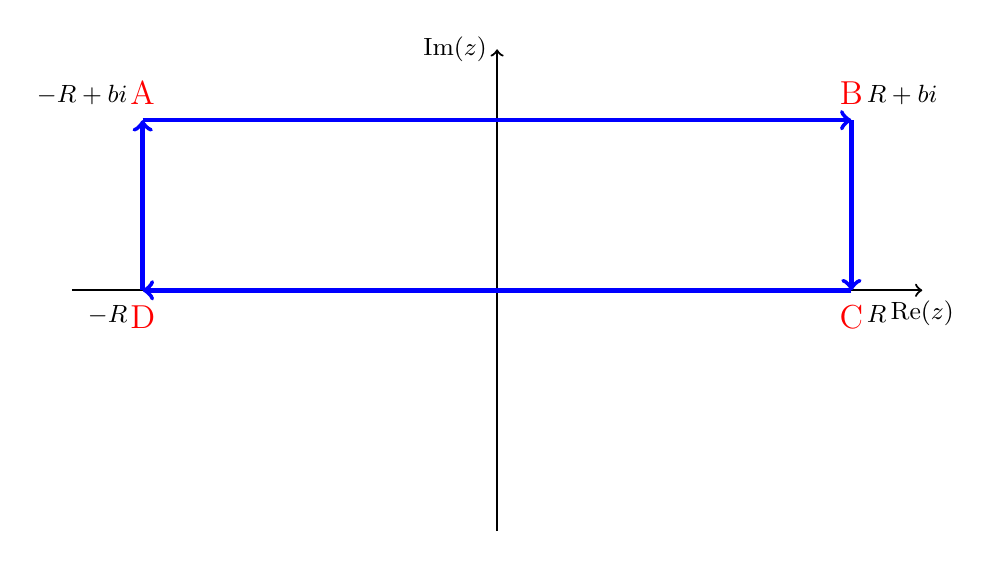
\begin{tikzpicture}[scale=1.8, font=\small]
				% Define coordinates
				\def\R{2.5}
				\def\b{1.2}
				
				% Draw axes
				\draw[->, thick] (-\R-0.5, 0) -- (\R+0.5, 0) node[below] {$\mathrm{Re}(z)$};
				% Adjusted y-axis to not overlap with labels
				\draw[->, thick] (0, -\b-0.5) -- (0, \b+0.5) node[left] {$\mathrm{Im}(z)$};
				
				% Define the vertex coordinates
				\coordinate (D) at (-\R, 0);
				\coordinate (C) at (\R, 0);
				\coordinate (B) at (\R, \b);
				\coordinate (A) at (-\R, \b);
				
				% --- MODIFICATION: Path labels C1, C2 etc. are removed ---
				% Draw paths with arrows only
				\draw[blue, ultra thick, ->] (C) -- (D);
				\draw[blue, ultra thick, ->] (B) -- (C);
				\draw[blue, ultra thick, ->] (A) -- (B);
				\draw[blue, ultra thick, ->] (D) -- (A);
				
				% Add vertex coordinate labels (black)
				\node[below left=2pt] at (D) {$-R$};
				\node[below right=2pt] at (C) {$R$};
				\node[above right=2pt] at (B) {$R+bi$};
				\node[above left=2pt] at (A) {$-R+bi$};
				
				% Add vertex letter labels (red), positioned to avoid overlap
				\node[red, above=2pt, font=\large] at (A) {A};
				\node[red, above=2pt, font=\large] at (B) {B};
				\node[red, below=2pt, font=\large] at (C) {C};
				\node[red, below=2pt, font=\large] at (D) {D};
				
			\end{tikzpicture}
		\end{center}
		
		根据柯西积分定理,函数在闭合围道上的积分为零:
		\begin{equation}\label{kexi}
			\oint_C e^{-az^2} dz = \int_{AB} e^{-az^2} dz + \int_{BC} e^{-az^2} dz + \int_{CD} e^{-az^2} dz + \int_{DA} e^{-az^2} dz = 0
		\end{equation}
		
		我们分别计算 $R \to \infty$ 时各段路径的积分。
		
		
		
		\textbf{1. 路径 $BC$ 与 $DA$:}
		在路径 $BC$ 上,参数化为 $z = R+iy$, $z(b) = R+ib$,$z(0) = R$,$dz=idy$, 其中 $y$ 从 $0$ 到 $b$。
		\begin{equation*}
			\left| \int_{BC} e^{-az^2} dz \right|= \left| \int_{R+bi}^{R} e^{-a(R+iy)^2} i dy \right|= \left| \int_{b}^{0} e^{-a(R+iy)^2} i dy \right| \le \int_{b}^{0} |e^{-a(R^2 - y^2 + 2iRy)}| dy 
		\end{equation*}
		\begin{equation*}
			= \int_{b}^{0} e^{-aR^2} e^{ay^2} dy = e^{-aR^2} \int_{b}^{0} e^{ay^2} dy
		\end{equation*}
		由于 $\int_{b}^{0} e^{ay^2} dy$ 是一个关于 $b$ 的常数,而 $\lim_{R \to \infty} e^{-aR^2} = 0$,所以:
		\begin{equation*}
			\lim_{R \to \infty} \left| \int_{BC} e^{-az^2} dz \right| = 0
		\end{equation*}
		同理可证,路径 $AD$ 的积分也为零。
		
		\textbf{2. 路径 $AB$:}
		在路径 $AB$ 上,参数化为 $z=x+bi$, $dz=dx$, 其中 $x$ 从 $R$ 变化到 $-R$。,由柯西积分公式\eqref{kexi}可知
		\begin{equation*}
			\int_{BA} e^{-az^2} dz = -	\int_{CD} e^{-az^2} dz = \int_{DC}e^{-az^2} dz= 	\lim_{R \to \infty}\int_{-R}^{R}e^{-ax^2} dx=\sqrt{\frac{\pi}{a}}
		\end{equation*}
		
		
		这证明了高斯积分的结果可以从实变量推广到复变量。
		
	\end{proof}
	
	
	
	
	\begin{example}\label{ex:3}
		$\int_{-\infty}^{+\infty} \cos kx \cdot e^{-a x^2} dx=\int_{-\infty}^{+\infty} e^{ikx} \cdot e^{-a x^2} dx= e^{-\frac{k^2}{4a}} \cdot \sqrt{\frac{\pi}{a}}$
	\end{example}
	
	\begin{proof}
		
		\begin{equation*}
			\int_{-\infty}^{+\infty} e^{ikx} \cdot e^{-a x^2} dx =\int_{-\infty}^{+\infty} \cos kx \cdot e^{-a x^2} dx+i\int_{-\infty}^{+\infty} \sin kx \cdot e^{-a x^2} dx
		\end{equation*}
		第二项为奇函数,积分为0,所以,
		\begin{equation*}
			\int_{-\infty}^{+\infty} e^{ikx} \cdot e^{-a x^2} dx =\int_{-\infty}^{+\infty} \cos kx \cdot e^{-a x^2} dx
		\end{equation*}
		
		\begin{equation*}
			\int_{-\infty}^{+\infty} e^{ikx} \cdot e^{-a x^2} dx = \int_{-\infty}^{+\infty} e^{-a x^2 + ikx} dx
		\end{equation*}
		
		配方
		\begin{equation*}
			\begin{split}
				-a x^2 + ikx &= -a \left( x^2 - \frac{ik}{a} x \right) \\
				&= -a \left[ x^2 - \frac{ik}{a} x + \left( \frac{ik}{2a} \right)^2 - \left( \frac{ik}{2a} \right)^2 \right] \\
				&= -a \left( x - \frac{ik}{2a} \right)^2 - \frac{k^2}{4a}
			\end{split}
		\end{equation*}
		所以,
		\begin{equation*}
			\int_{-\infty}^{+\infty} e^{ikx} \cdot e^{-a x^2} dx = \int_{-\infty}^{+\infty} e^{-a x^2 + ikx} dx	= e^{-\frac{k^2}{4a}} \cdot \sqrt{\frac{\pi}{a}}
		\end{equation*}
	\end{proof}
	
	
	\begin{example}\label{ex:4}
		$\int_{-\infty}^{+\infty} z^2 e^{-a z^2} dz = \frac{1}{2} \pi^{\frac{1}{2}} a^{-\frac{3}{2}}$
	\end{example}
	
	\begin{proof}
		
		
		\begin{equation*}
			\text{设} \quad \Phi(a) = \int_{-\infty}^{+\infty} e^{-a z^2} dz = \sqrt{\frac{\pi}{a}}
		\end{equation*}
		
		\begin{equation*}
			\frac{d\Phi}{da} = -\int_{-\infty}^{+\infty} z^2 e^{-a z^2} dz = \frac{d}{da} \left( \pi^{\frac{1}{2}} a^{-\frac{1}{2}} \right) = \pi^{\frac{1}{2}} a^{-\frac{3}{2}} \cdot \left( -\frac{1}{2} \right)
		\end{equation*}
		
		\begin{equation*}
			\therefore \int_{-\infty}^{+\infty} z^2 e^{-a z^2} dz = \frac{1}{2} \pi^{\frac{1}{2}} a^{-\frac{3}{2}}
		\end{equation*}
	\end{proof}
	
	
	
	\begin{example}\label{ex:5}
		$	\int_{-\infty}^{+\infty} (z + bx)^2 e^{-a z^2} dz=	= \frac{1}{2} \pi^{\frac{1}{2}} a^{-\frac{3}{2}} + b^2 x^2 \sqrt{\frac{\pi}{a}}$
	\end{example}
	
	\begin{proof}
		展开得
		\begin{equation*}
			= \int_{-\infty}^{+\infty} z^2 e^{-a z^2} dz + \int_{-\infty}^{+\infty} 2 z b x e^{-a z^2} dz + b^2 x^2 \int_{-\infty}^{+\infty} e^{-a z^2} dz
		\end{equation*}
		
		\begin{equation*}
			= \frac{1}{2} \pi^{\frac{1}{2}} a^{-\frac{3}{2}} + b^2 x^2 \sqrt{\frac{\pi}{a}}
		\end{equation*}
		
	\end{proof}
	
	
	
	
	
	
	
	
	\subsection{解的导出}
	对于无界的热传导方程\eqref{wujierechuandao}:
	\begin{equation}
		\begin{cases}
			u_t - a\Delta u = 0, \\
			u(x, 0) = \varphi(x),
		\end{cases}
	\end{equation}
	
	设初值问题的解 \( u(x, t) \) 和初始数据 \( \varphi(x) \) 都可关于变量 \( x \) 进行 Fourier 变换,并记:
	\begin{equation}
		\hat{u}(\xi, t) = \int_{\mathbb{R}^n} u(x, t) e^{-i x \cdot \xi} dx,
	\end{equation}
	\begin{equation}
		\hat{\varphi}(\xi) = \int_{\mathbb{R}^n} \varphi(x) e^{-i x \cdot \xi} dx.
	\end{equation}
	
	对热传导方程和初始条件进行 Fourier 变换,根据傅里叶的微分性质\eqref{weifen}:
	\begin{equation}
		\hat{u_t}=\int_{\mathbb{R}^n} u_t(x, t) e^{-i x \cdot \xi} dx=\frac{d}{dt} \int_{\mathbb{R}^n} u(x, t) e^{-i x \cdot \xi} dx= \frac{d\hat{u}(\xi, t)}{dt}
	\end{equation}
	
	\[
	\Delta u = \sum_{j=1}^n \frac{\partial^2 u}{\partial x_j^2}
	\]
	\[
	\mathcal{F}\left[\frac{\partial^2 u}{\partial x_j^2}\right](\xi) = -\xi_j^2 \hat{u}(\xi)
	\]
	\begin{equation}
		\mathcal{F}[\Delta u](\xi) = \sum_{j=1}^n (-\xi_j^2) \hat{u}(\xi) = -|\xi|^2 \hat{u}(\xi)
	\end{equation}
	
	
	把$\xi$看作常量,得到关于 \(\hat{u}(\xi, t)\) 的常微分方程初值问题:
	\begin{equation}
		\begin{cases}
			\displaystyle \frac{d\hat{u}(\xi, t)}{dt} + a|\xi|^2 \hat{u}(\xi, t) = 0, \\
			\hat{u}(\xi, 0) = \hat{\varphi}(\xi).
		\end{cases}
	\end{equation}
	该方程的解为:
	\begin{equation}
		\hat{u}(\xi, t) = \hat{\varphi}(\xi) e^{-a|\xi|^2 t}.
	\end{equation}
	
	
	
	\begin{proof}
		这是一个一阶线性常微分方程,可以通过分离变量法求解。
		将方程改写为:
		\[
		\frac{d\hat{u}}{\hat{u}} = -a |\xi|^2 dt
		\]
		
		对两边积分:
		\[
		\int \frac{d\hat{u}}{\hat{u}} = \int -a |\xi|^2 dt
		\]
		
		得到:
		\[
		\ln|\hat{u}| = -a |\xi|^2 t + C(\xi)
		\]
		其中,\(C(\xi)\) 是积分常数,可能依赖于 \(\xi\)。
		
		
		利用初始条件 \(\hat{u}(\xi, 0) = \hat{\varphi}(\xi)\),代入上式得:
		\[
		C(\xi) = \ln|\hat{\varphi}(\xi)|
		\]
		
		将 \(C(\xi)\) 代入积分结果:
		\[
		\ln|\hat{u}| = -a |\xi|^2 t + \ln|\hat{\varphi}(\xi)|
		\]
		
		对两边取指数:
		\[
		\hat{u}(\xi, t) = \hat{\varphi}(\xi) e^{-a |\xi|^2 t}
		\]
		
		
	\end{proof}
	
	
	对 \(\hat{u}(\xi, t)\) 进行 Fourier 逆变换
	\begin{equation}
		u(x, t) = \mathcal{F}^{-1}[\hat{\varphi}(\xi) e^{-a|\xi|^2 t}]
	\end{equation}
	
	利用Fourier 逆变换卷积的性质\eqref{nibianhuanjuanji}:
	\begin{equation}
		u(x, t) = \mathcal{F}^{-1}[\hat{\varphi}(\xi)] * \mathcal{F}^{-1}[e^{-a|\xi|^2 t}]
	\end{equation}
	
	\begin{example}
		我们需要证明:
		\[
		\mathcal{F}^{-1}\left[e^{-a|\xi|^2 t}\right](x) = (4\pi a t)^{-n/2} e^{-\frac{|x|^2}{4a t}}
		\]
	\end{example}
	
	
	
	\begin{proof}
		
		根据傅里叶逆变换的定义:
		\[
		\mathcal{F}^{-1}\left[e^{-a|\xi|^2 t}\right](x) = \frac{1}{(2\pi)^n} \int_{\mathbb{R}^n} e^{i x \cdot \xi} e^{-a|\xi|^2 t} d\xi
		\]
		
		我们可以将这个积分分解为每个坐标的积分:
		\[
		\mathcal{F}^{-1}\left[e^{-a|\xi|^2 t}\right](x) = \frac{1}{(2\pi)^n} \prod_{j=1}^n \int_{-\infty}^\infty e^{i x_j \xi_j} e^{-a\xi_j^2 t} d\xi_j
		\]
		
		\begin{remark}
			\[
			\mathcal{F}^{-1}\left[e^{-a|\xi|^{2} t}\right](x)=\frac{1}{(2\pi)^{n}}\prod_{j=1}^{n}\left(\int_{-\infty}^{\infty} e^{i x_j \xi_j} e^{-a\xi_j^{2} t} d\xi_j\right)
			\]
		\end{remark}
		
		
		对于每个一维积分,我们有:
		\[
		\int_{-\infty}^\infty e^{i x_j \xi_j} e^{-a\xi_j^2 t} d\xi_j
		\]
		
		对指数部分进行配方:
		\[
		-a t \xi_j^2 + i x_j \xi_j = -a t \left( \xi_j^2 - \frac{i x_j}{a t} \xi_j \right)
		\]
		\[
		= -a t \left( \xi_j^2 - \frac{i x_j}{a t} \xi_j + \left( \frac{x_j}{2a t} \right)^2 - \left( \frac{x_j}{2a t} \right)^2 \right)
		\]
		\[
		= -a t \left( \left( \xi_j - \frac{i x_j}{2a t} \right)^2 - \frac{x_j^2}{4a^2 t^2} \right)
		\]
		\[
		= -a t \left( \xi_j - \frac{i x_j}{2a t} \right)^2 + \frac{x_j^2}{4a t}
		\]
		
		代入积分中,由命题\eqref{ex:1}:
		\[
		\int_{-\infty}^\infty e^{-a t \left( \xi_j - \frac{i x_j}{2a t} \right)^2 + \frac{x_j^2}{4a t}} d\xi_j = e^{\frac{x_j^2}{4a t}} \int_{-\infty}^\infty e^{-a t \left( \xi_j - \frac{i x_j}{2a t} \right)^2} d\xi_j= \sqrt{\frac{\pi}{a t}} e^{\frac{x_j^2}{4a t}}
		\]
		
		
		将所有坐标的结果相乘,并乘以系数 \( \frac{1}{(2\pi)^n} \),得到:
		\[
		\mathcal{F}^{-1}\left[e^{-a|\xi|^2 t}\right](x) = \frac{1}{(2\pi)^n} \left( \sqrt{\frac{\pi}{a t}} \right)^n e^{-\frac{|x|^2}{4a t}}
		\]
		\[
		= \frac{1}{(2\pi)^n} \cdot \frac{\pi^{n/2}}{(a t)^{n/2}} e^{-\frac{|x|^2}{4a t}} = (4\pi a t)^{-n/2} e^{-\frac{|x|^2}{4a t}}
		\]
		
	\end{proof}
	
	
	
	
	
	因此,解可以表示为:
	\begin{equation}
		u(x, t) = (4\pi a t)^{-n/2} \int_{\mathbb{R}^n} \varphi(y) e^{-\frac{|x - y|^2}{4a t}} dy
	\end{equation}
	

	
		\newpage
	\section{无界非齐次热传导方程}
	和之前波动方程齐次化一样,先用叠加原理分解成两个子问题,用Duhamamel原理把方程齐次化。
	
	对于无界基础方程,把基本解看作达朗贝尔公式。
	
	\section{半直线热传导方程}
	把无界基础方程的基本解(泊松公式)看作达朗贝尔公式,第一边界用奇延拓,第二边界用偶延拓。
	
	
	\section{有界非齐次热传导方程}
	先用叠加原理分解成三个子问题,用Duhamamel原理把方程齐次化,用插值边界齐次化。
	
	对于有界基本方程用分离变量法,过程和波动的一样,就是时间常微分函数变成一阶通解为指数函数,而不再是三角函数。系数由边界条件决定,其他全部的求解过程,验证过程全部一样。
	
	也可以像达朗贝尔公式那样,满足相容性条件做奇偶延拓,再做周期延拓。
	\href{https://kns.cnki.net/kcms2/article/abstract?v=VQ0ntgfwFMTzN6hnFDpFMFM9DxAtYwMQhco2QSA-IEHGx9q5EylUyfVfvJ65vLbYgxi4GKWYtrw0WYFjulce4L-QdEJiwrbko6gMtLg1u_v-yZO9l1KqPNK5VVy0WXMK_iyRkdOb_3JYM79j78dC5ZO49R0B00eT_N_tEe4_tT88MKGKuKknjw==&uniplatform=NZKPT&language=CHS}{偏微分方程课程研究型教学的一个实例剖析,朱长江}
	
	
	%弱解
%	\href{https://en.wikipedia.org/wiki/Weak_solution}{(Weak Solution)}
	
	
	
\end{document}